\documentclass[12pt]{article}  % [12pt] option for the benefit of aging markers

% amssymb package contains more mathematical symbols
\usepackage{amssymb,amsthm}
\usepackage{amsmath}

% graphicx package enables you to paste in graphics
\usepackage{graphicx}
\usepackage{auto-pst-pdf}
\usepackage{subfig}

% embed source inside latex
\usepackage[procnames]{listings}
\usepackage{color}

% page geometry
\usepackage{geometry}
\usepackage{array}

% ALGORITHM
\usepackage{algorithm}
\usepackage{algpseudocode}
\usepackage{hyperref}
\usepackage{booktabs}
\usepackage{enumitem}

%%%%%%%%%%%%%%%%%%%%%%%%%%%%%%%%%
%
%    Page size commands.  Don't worry about these
%
\setlength{\textheight}{220mm}
\setlength{\topmargin}{-10mm}
\setlength{\textwidth}{150mm}
\setlength{\oddsidemargin}{0mm}

%%%%%%%%%%%%%%%%%%%%%%%%%%%%%%%%%%%%%%%%%%%%%%%%%%%%%%%%%%%%%%%
%
%    Definitions of environments for theorems etc.
%
\newtheorem{theorem}{Theorem}[section]          % Theorems numbered within sections - eg Theorem 2.1 in Section 2.
\newtheorem{corollary}[theorem]{Corollary}      % Corollaries etc. will be counted as Theorems for numbering
\newtheorem{lemma}[theorem]{Lemma}              % eg Lemma 3.1, ... Theorem 3.2, ... Corollary 3.3.
\newtheorem{proposition}[theorem]{Proposition}
\newtheorem{conjecture}[theorem]{Conjecture}

\theoremstyle{definition}
\newtheorem{definition}[theorem]{Definition}

\theoremstyle{remark}
\newtheorem{remark}[theorem]{Remark}
\newtheorem{example}[theorem]{Example} 

%%%%%%%%%%%%%%%%%%%%%%%%%%%%%%%%%%%%%%%%%%%%%%%
%
%        Preamble material specific to your essay
%
\title{Modeling and Active Inferring Wireless Sensor Data}
\author{Yan Jiaqi A20321362\\
CS583 Project\\
supervised by
Mustafa Bilgic\\
Live Section
}

\begin{document}
\maketitle

% \newpage                     % optional page break
\begin{abstract}
Phase 1
\end{abstract}

% optional page break
\newpage
\tableofcontents

% optional page break
\newpage
\section{Phase 1 Experiment Results}
\label{sec:des}

\begin{figure}[h]
\centering
        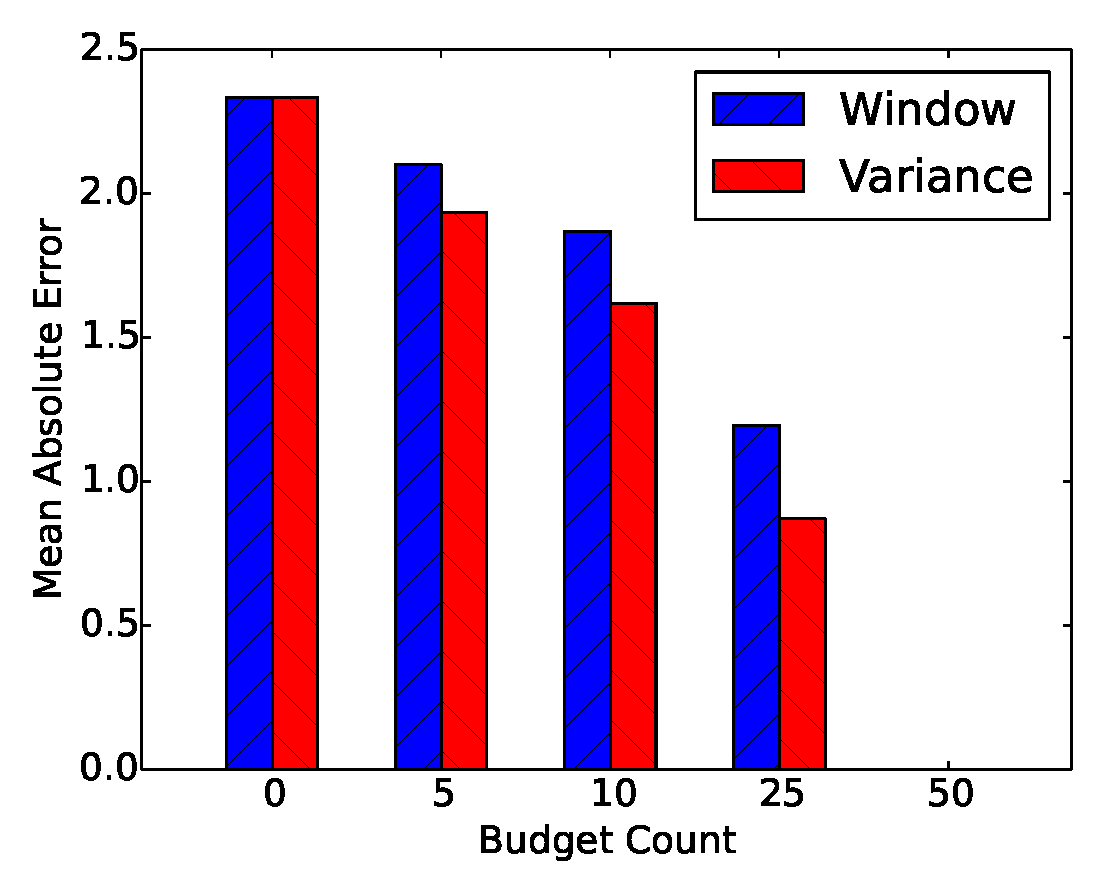
\includegraphics[width=0.58\textwidth]{../temperature_err}
\caption{Inference Errors of Temperature Data at Different Budget Level}
\label{fig:phase1:temperature}
\end{figure}

\begin{figure}[h]
\centering
        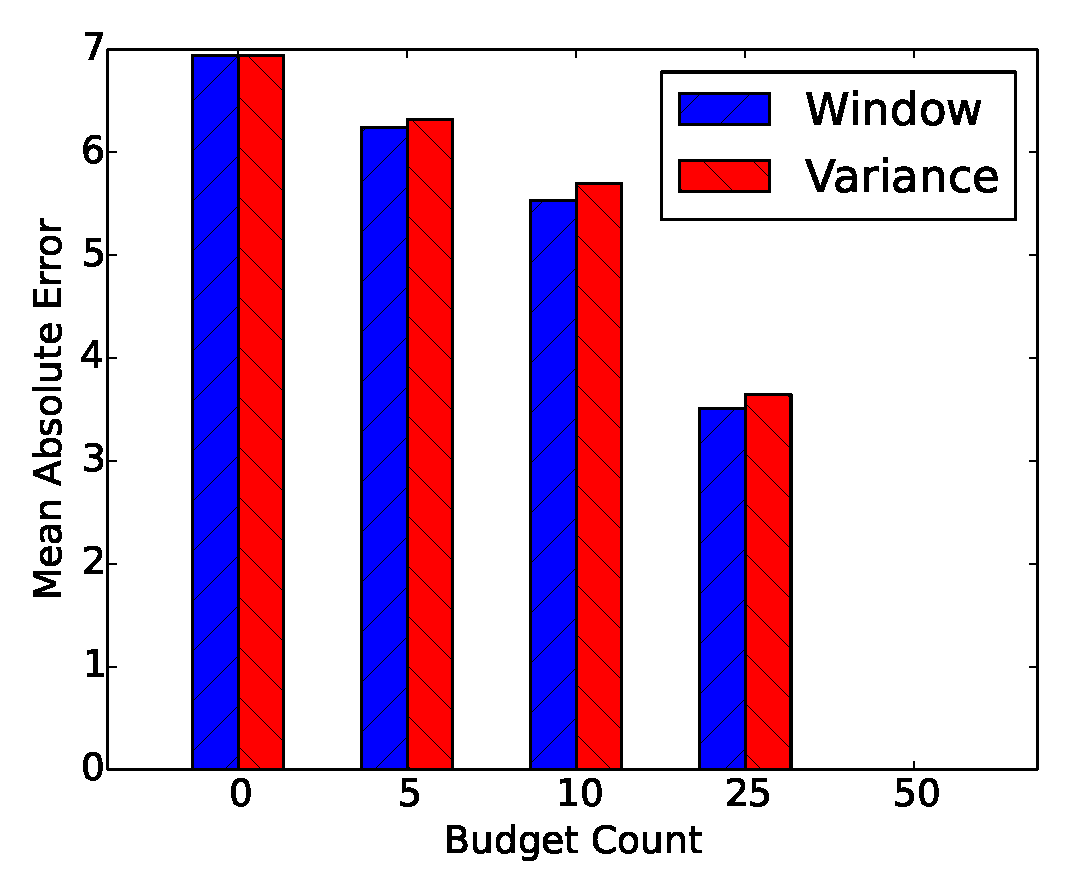
\includegraphics[width=0.58\textwidth]{../humidity_err}
\caption{Inference Errors of Humidity Data at Different Budget Level}
\label{fig:phase1:humidity}
\end{figure}

%\begin{figure}[h]
%\centering
        %\includegraphics[width=0.8\textwidth, height=0.8\textheight]{progress.ps}
%\caption{Discovery Percentage as Function of Iteration for $R_1$ and $R_6$}
%\label{fig:progress}
%\end{figure}


%%%%%%%%%%%%%%%%%%%%%%%%%%%%%%%%%%%%%%%%%
%
%     Bibliography
%
%     Use an easy-to-remember tag for each entry - eg \bibitem{How97} for an article/book by Howie in 1997
%     To cite this publication in your text, write \cite{How97}.  To include more details such as
%     page, Chapter, Theorem numbers, use the form \cite[Theorem 6.3, page 42]{How97}.
%
%\begin{thebibliography}{99}

% 
% The usual convention for mathematical bibliographies is to list alphabetically
% by first-named author (then second, third  etc. author then date)
% websites with no author names should go by the site name
%


% Typical layout for reference to a journal article
%
%\bibitem{Bovey}
%J. D. Bovey, M. M. Dodson,                         % author(s)
%The Hausdorff dimension of systems of linear forms % article name
%{\em Acta Arithmetica}                             % journal name - italics
%{\bf 45}                                           % volume number - bold
%(1986), 337--358.                                   % (year), page range

%% Typical layout for reference to a book
%%
%\bibitem{Cassels}
%J. W. S. Cassels,                                  % author(s)
%{\em An Introduction to Diophantine Approximation},% title - italics
%Cambridge University Press, Cambridge, 1965.       % Publisher, place, date.

%% Typical layout for reference to a website
%%
%\bibitem{GAP}
%The GAP Group, GAP -- Groups, Algorithms, and Programming,  % Site name
%Version 4.5.6; 2012. % other information
%(http://www.gap-system.org)  % URL


%% Typical layout for reference to an online article
%%
%\bibitem{Howie}
%J. Howie,                                            % author(s)
%{\em Generalised triangle groups of type $(3,5,2)$}, % article name - italics
%http://arxiv.org/abs/1102.2073                       % URL
%(2011).                                              % (year)
%\end{thebibliography}

\end{document}
